\documentclass[xcolor=dvipsnames]{beamer}
\usepackage{amsmath}
\usepackage{hyperref}
\usepackage{ragged2e}
\usepackage{graphicx}
\usetheme{Copenhagen}
\usecolortheme[named=Black]{structure}

\title{BRIEF: Computing a Local Binary Descriptor Very Fast}
\author{Castleberry, Cherry, and Firth}
\renewcommand{\raggedright}{\leftskip=0pt \rightskip=0pt plus 0cm}

\begin{document}

\maketitle
\section{Introduction}
\subsection{Motivation}

\frame{\frametitle{Motivation: A 256-Byte Descriptor?}
 \begin{figure}
  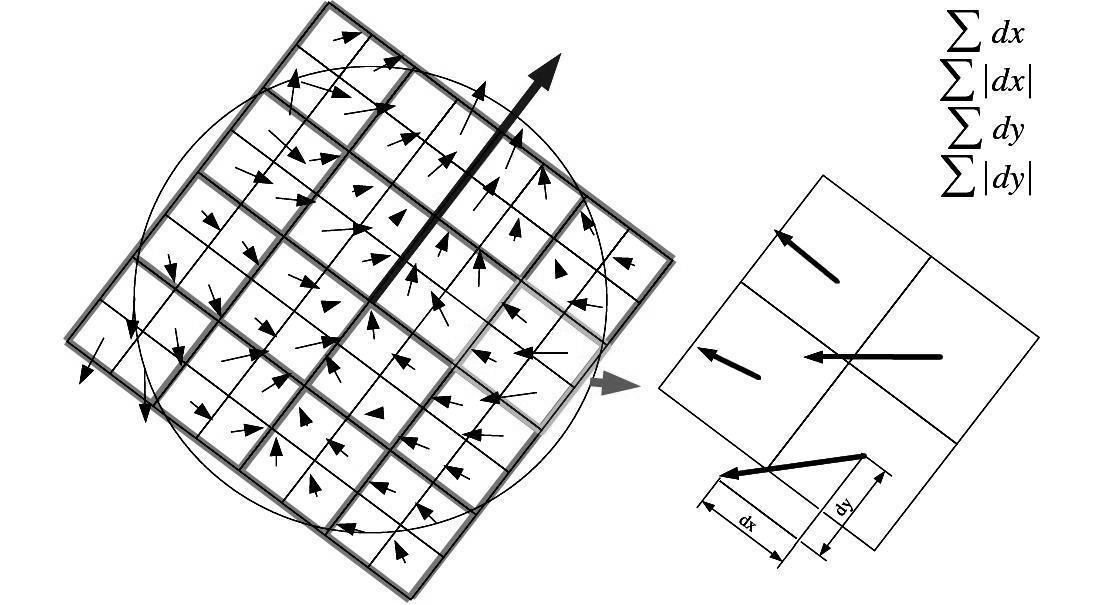
\includegraphics[width=\textwidth]{imgs/256-bytes.jpg}
  \caption{A SURF descriptor stores 64 orientation values as 4-byte integers.}
 \end{figure}
}

\subsection{Problem Definition}

\frame{\frametitle{Problem Definition: Make It Smaller, Compute It Faster}
 \setlength{\unitlength}{1mm}
 \begin{center}
 \begin{figure}
 \begin{picture}(30,30)
  \put(0,0 ){\circle*{5}} 
  \put(0,8 ){\circle*{5}} 
  \put(0,16){\circle*{5}} 
  \put(0,24){\circle*{5}} 
  \put(8,0 ){\circle*{5}} 
  \put(8,8 ){\circle*{5}} 
  \put(8,16){\circle*{5}} 
  \put(8,24){\circle*{5}} 
  \put(30,12){\circle*{5}} 
 \end{picture}
 \vspace{12pt}
 \caption{Reduce the size by a factor of 8.}
 \end{figure}
 \end{center}
}

\subsection{Previous Work}

\frame{\frametitle{Previous Work: Principal Component Analysis}
 \begin{figure}
  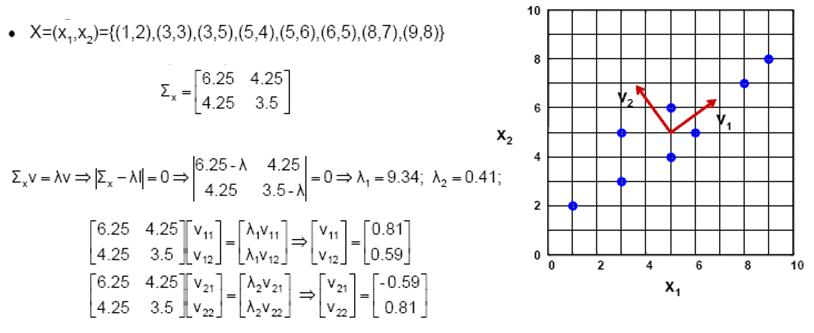
\includegraphics[width=1.0\textwidth]{imgs/pca_example.png}
 \end{figure}
}

\frame{\frametitle{Previous Work: Floating-Point Quantization}
 \begin{figure}
  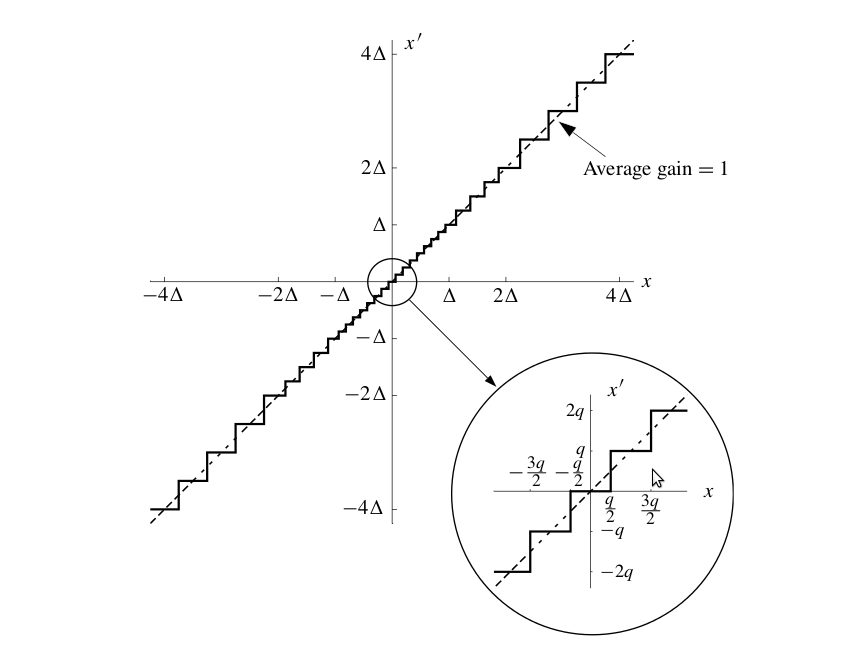
\includegraphics[width=.7\textwidth]{imgs/quantizer.png}
  \caption{Quantization with a 3-Bit Mantissa.}
 \end{figure}
}

\subsection{Background}

\frame{ \frametitle{Background: Hamming Distance}
  \begin{center}
  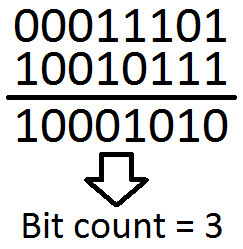
\includegraphics[width=.5\textwidth]{imgs/hamming.png}
  \end{center}
}

\frame{ \frametitle{Background: Hamming Distance}
  \begin{center}
  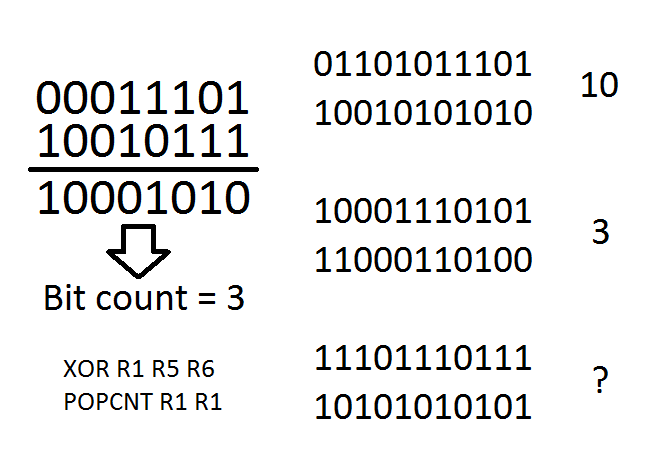
\includegraphics[width=.7\textwidth]{imgs/hamming2.png}
  \end{center}
}

\section{Method}

\subsection{Techniques Used}
\subsection{Method}

\frame{\frametitle{Method: Sampling Distributions}
 \begin{figure}
  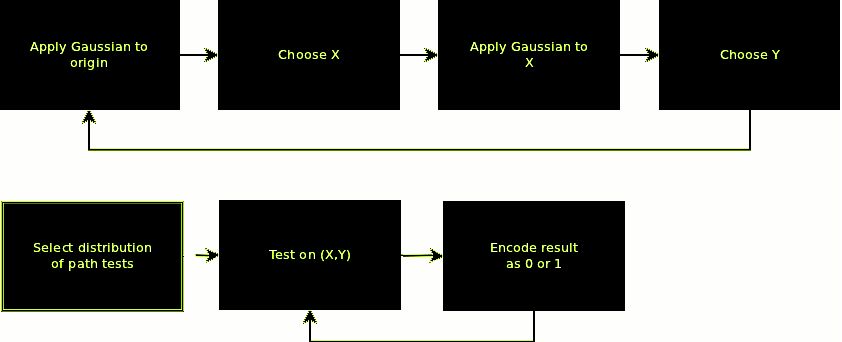
\includegraphics[width=\textwidth]{imgs/workflow.png}
  \caption{Sampling distributions.}
 \end{figure}
}

\frame{\frametitle{Method: Patch Test}
 \begin{equation}
  \tau (p; \mathbf{x},y) :=
  \begin{Bmatrix}
   1 & \text{if}\ I(\mathbf{p},\mathbf{x}) < I(\mathbf{p},\mathbf{y}) \\
   0 & \text{otherwise}
  \end{Bmatrix}
 \end{equation}
}

\frame{\frametitle{Method: Descriptor Formula}
 \begin{equation}
  \sum_{I \leq i \leq n_d} 2^{i-1} \tau(p; x_i, y_i)
 \end{equation}
}


\frame{\frametitle{Method: Example of Distribution}
 \begin{figure}
  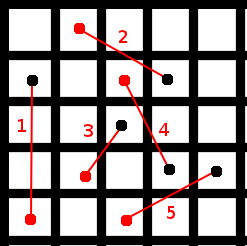
\includegraphics[width=.6\textwidth]{imgs/grid.png}
  \caption{Sampling distributions.}
 \end{figure}
}

\frame{\frametitle{Example of Patch Test on Distribution}
\begin{minipage}{.45\linewidth}
%\begin{flushleft}
\begin{center}
\[
 \begin{bmatrix}
  1 & 3 & 5 & 4 & 2 \\ 
  3 & 2 & 1 & 8 & 7 \\ 
  9 & 5 & 4 & 6 & 4 \\
  7 & 9 & 5 & 2 & 1 \\
  2 & 3 & 6 & 5 & 4 
 \end{bmatrix}
\]
 \begin{figure}
  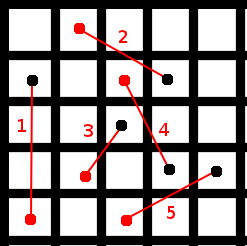
\includegraphics[width=.5\textwidth]{imgs/grid.png}
  \caption{Sampling distributions.}
 \end{figure}
\end{center}
%\end{flushleft}
\end{minipage}
\begin{minipage}{.45\linewidth}
%\begin{flushright}
\begin{center}
\begin{tabular}{ll|r}
 x & y & $\tau$ \\ \hline
 2 & 3 & 1 \\ 
 3 & 8 & 1 \\ 
 9 & 4 & 0 \\ 
 1 & 2 & 1 \\ 
 6 & 1 & 0 
\end{tabular}
\\
\vspace{12pt}
11010
\end{center}
%\end{flushright}
\end{minipage}
}

\frame{\frametitle{Example of Patch Test on Distribution}
\begin{minipage}{.45\linewidth}
%\begin{flushleft}
\begin{center}
\[
 \begin{bmatrix}
  3 & 2 & 1 & 8 & 7 \\ 
  9 & 5 & 4 & 6 & 4 \\
  7 & 9 & 5 & 2 & 1 \\
  1 & 3 & 5 & 4 & 2 \\ 
  2 & 3 & 6 & 5 & 4 
 \end{bmatrix}
\]
 \begin{figure}
  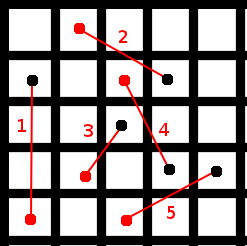
\includegraphics[width=.5\textwidth]{imgs/grid.png}
  \caption{Sampling distributions.}
 \end{figure}
\end{center}
%\end{flushleft}
\end{minipage}
\begin{minipage}{.45\linewidth}
%\begin{flushright}
\begin{center}
\begin{tabular}{ll|r}
 x & y & $\tau$ \\ \hline
 2 & 9 & 1 \\ 
 2 & 6 & 1 \\ 
 3 & 5 & 1 \\ 
 4 & 4 & 0 \\ 
 6 & 2 & 0 
\end{tabular}
\\
\vspace{12pt}
11100
\end{center}
%\end{flushright}
\end{minipage}
}

\frame{\frametitle{}
\begin{center}
\begin{tabular}{ccccc}
 1 & 1 & 0 & 1 & 0 \\ 
 1 & 1 & 1 & 0 & 0 \\ 
 y & y & n & n & y  
\end{tabular}
\\
\vspace{12pt}
 Hamming distance: 2.
\end{center}
}

\frame{\frametitle{Method: Sampling}
 \begin{figure}
  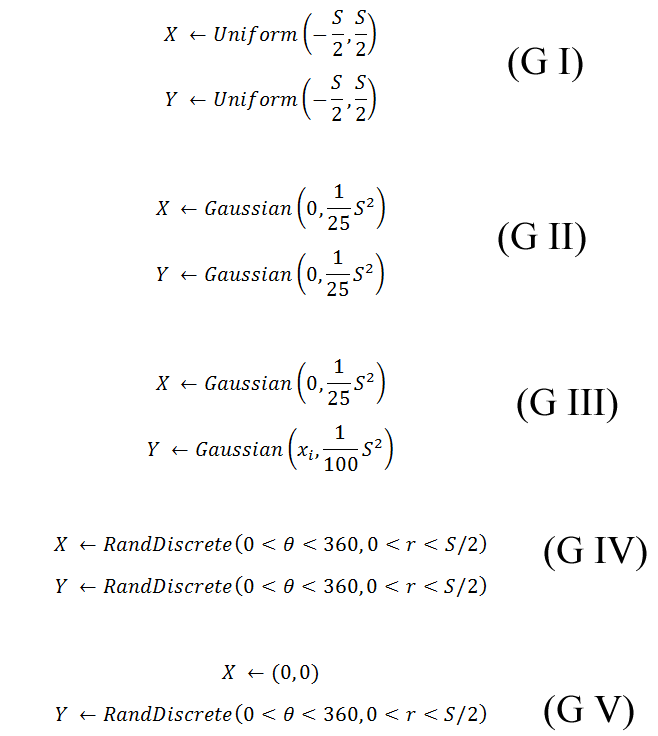
\includegraphics[width=.5\textwidth]{imgs/spat_dist.png}
 \end{figure}
}

\frame{\frametitle{Method: Sampling Distributions}
 \begin{figure}
  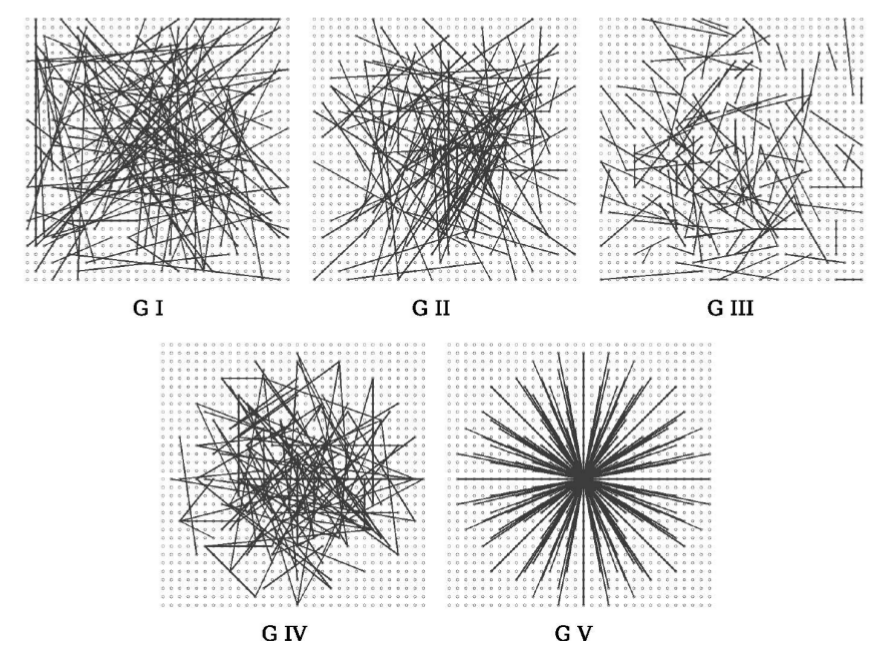
\includegraphics[width=.75\textwidth]{imgs/sampling.png}
  \caption{Sampling distributions.}
 \end{figure}
}

\subsection{Data}

\frame{\frametitle{} 
       \begin{center} 
       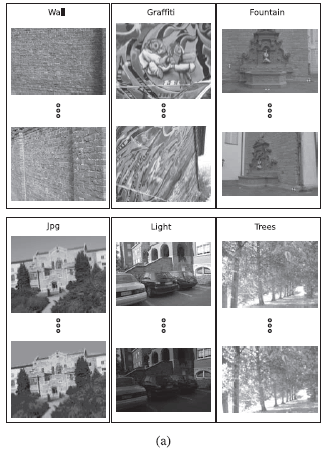
\includegraphics[width=.5\textwidth]{imgs/figure10a.png} 
       \end{center} 
      }
\frame{\frametitle{} 
       \begin{center} 
       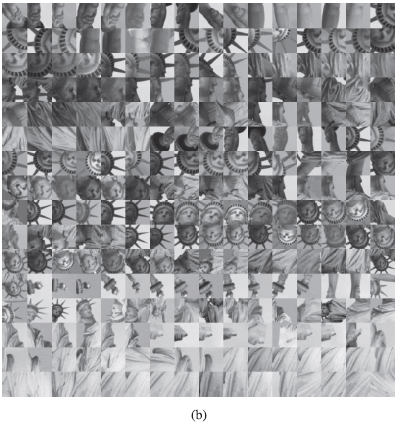
\includegraphics[width=.7\textwidth]{imgs/figure10b.png} 
       \end{center} 
      }


\subsection{Experimental Setup}
\frame{ \frametitle{Experimental Setup}
\begin{itemize}
 \item U-BRIEF
 \item S-BRIEF
 \item O-BRIEF
 \item D-BRIEF
\end{itemize} 
}

\section{Conclusion}
\subsection{Results}

\frame{\frametitle{} 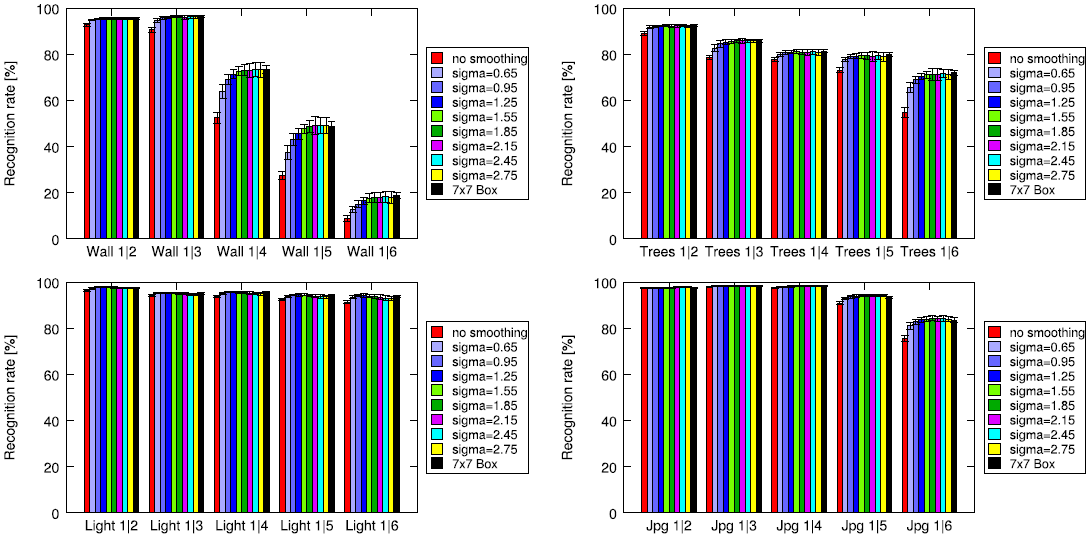
\includegraphics[width=\textwidth]{imgs/figure01.png} }
\frame{\frametitle{} 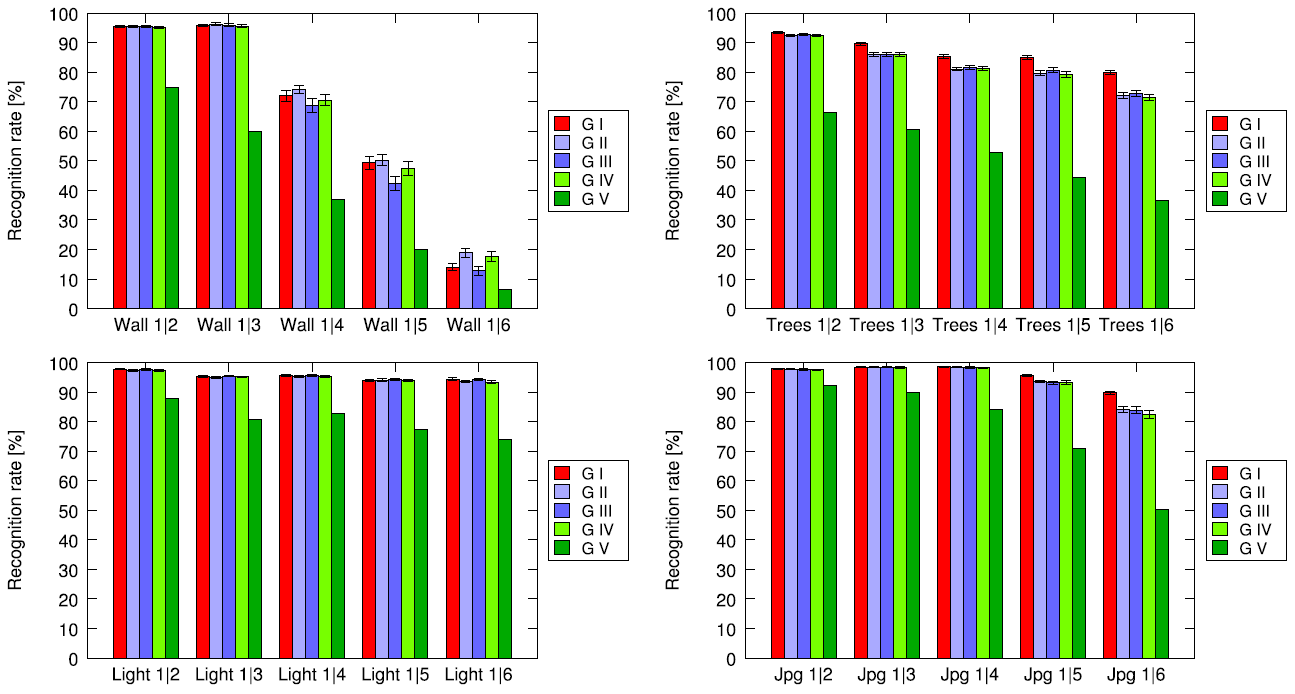
\includegraphics[width=\textwidth]{imgs/figure03.png} }
\frame{\frametitle{} 
       \begin{center} 
       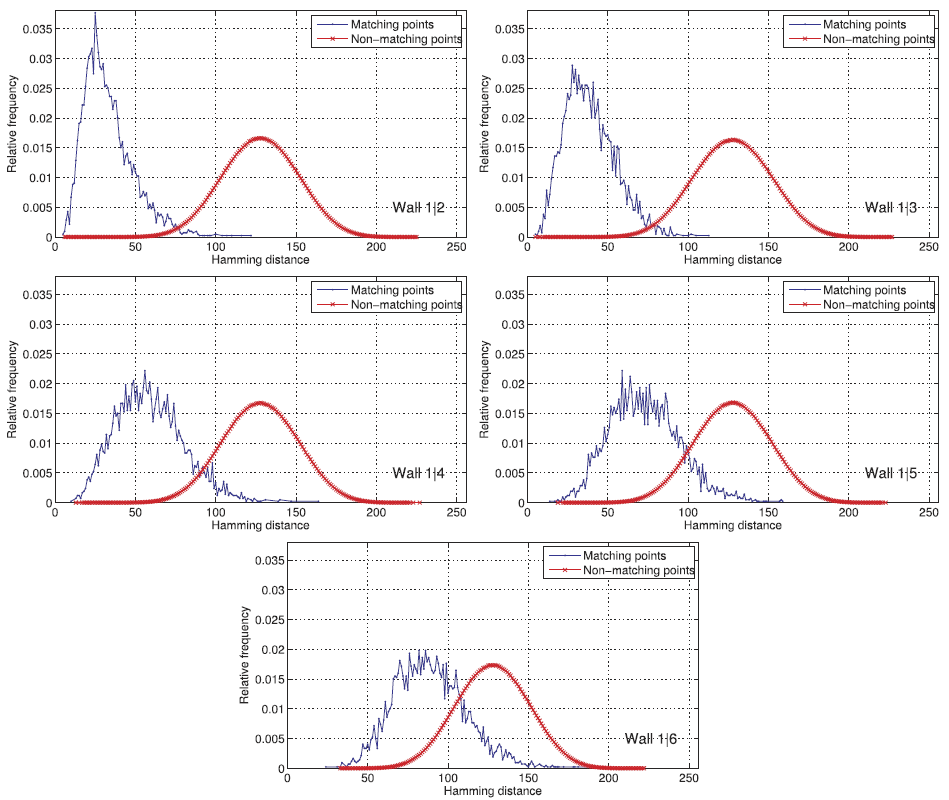
\includegraphics[width=.7\textwidth]{imgs/figure04.png} 
       \end{center} 
      }
\frame{\frametitle{} 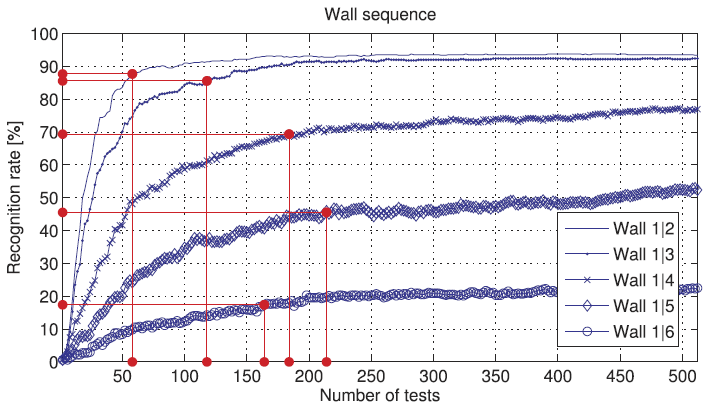
\includegraphics[width=\textwidth]{imgs/figure05.png} }
\frame{\frametitle{} 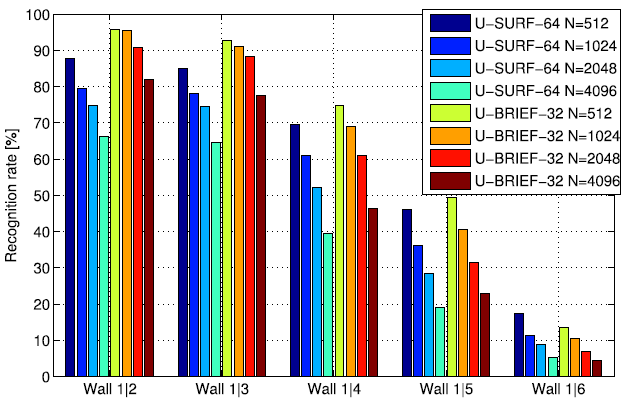
\includegraphics[width=\textwidth]{imgs/figure06.png} }
\frame{\frametitle{} 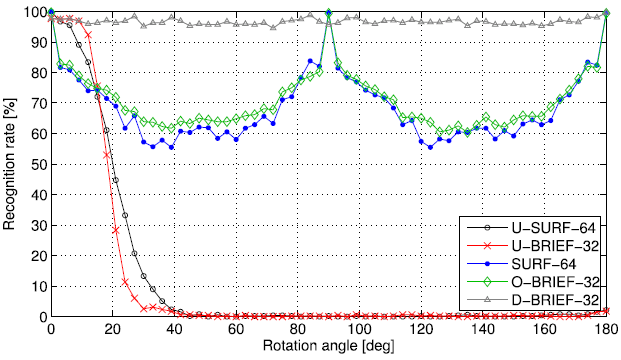
\includegraphics[width=\textwidth]{imgs/figure07.png} }
\frame{\frametitle{} 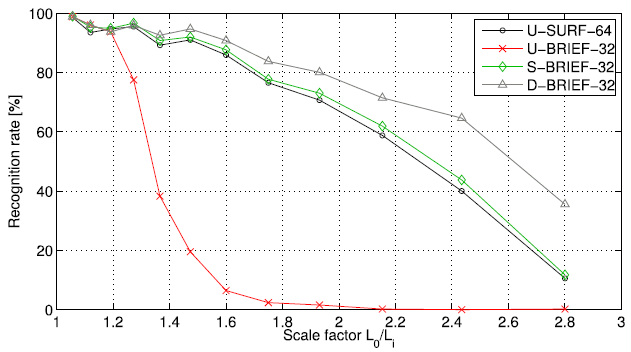
\includegraphics[width=\textwidth]{imgs/figure08.png} }
\frame{\frametitle{} 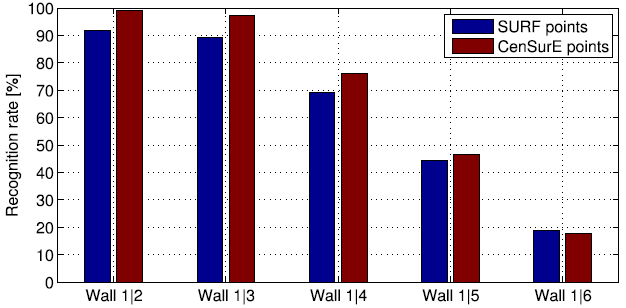
\includegraphics[width=\textwidth]{imgs/figure09.png} }
\frame{\frametitle{} 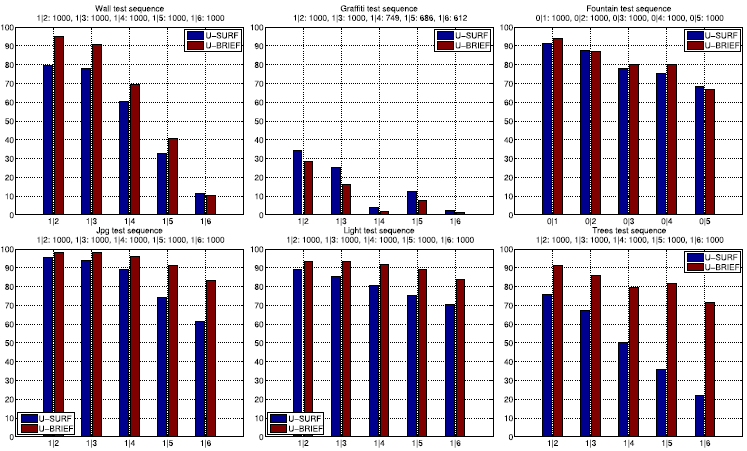
\includegraphics[width=\textwidth]{imgs/figure11.png} }
\frame{\frametitle{} 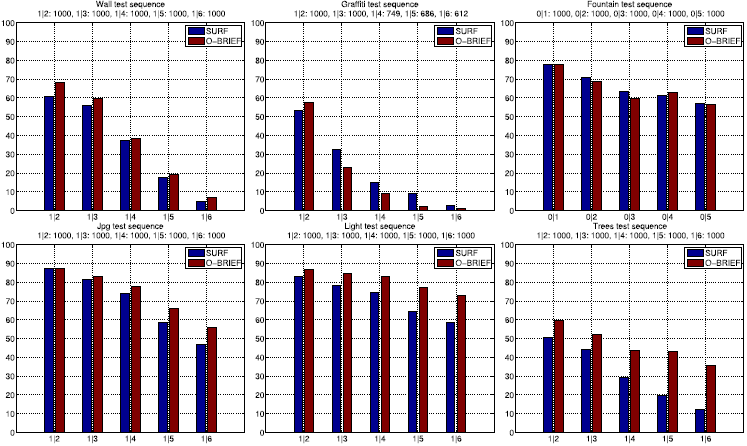
\includegraphics[width=\textwidth]{imgs/figure12.png} }
\frame{\frametitle{} 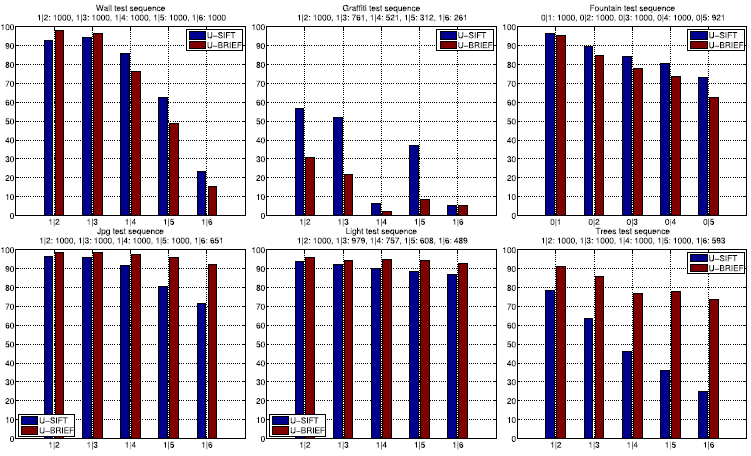
\includegraphics[width=\textwidth]{imgs/figure13.png} }
\frame{\frametitle{} 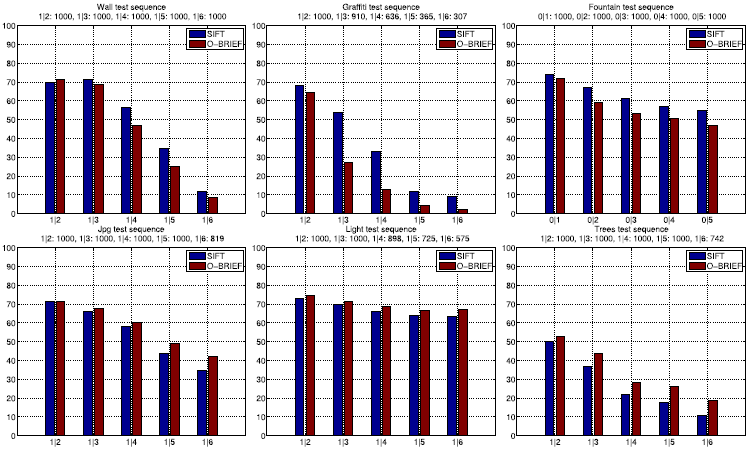
\includegraphics[width=\textwidth]{imgs/figure14.png} }
\frame{\frametitle{} 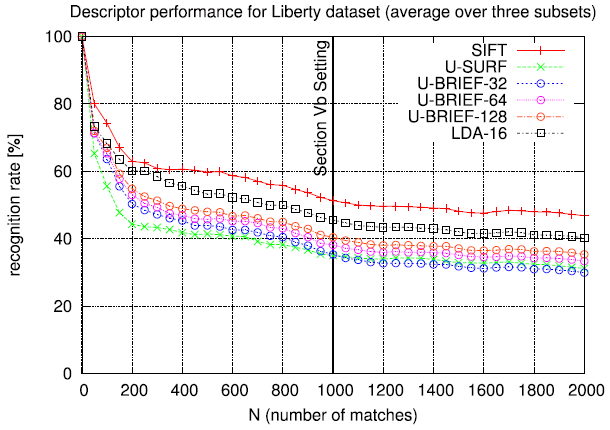
\includegraphics[width=\textwidth]{imgs/figure15.png} }
\frame{\frametitle{} 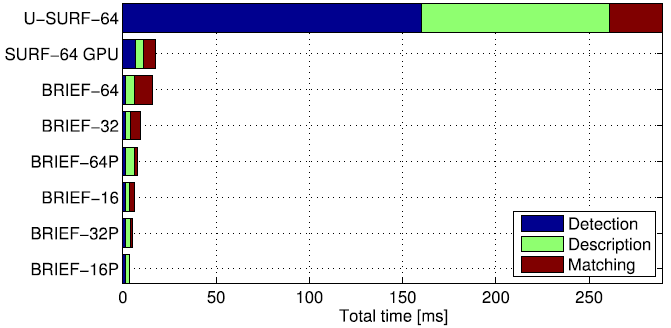
\includegraphics[width=\textwidth]{imgs/figure16.png} }
\frame{\frametitle{} 
       \begin{center} 
       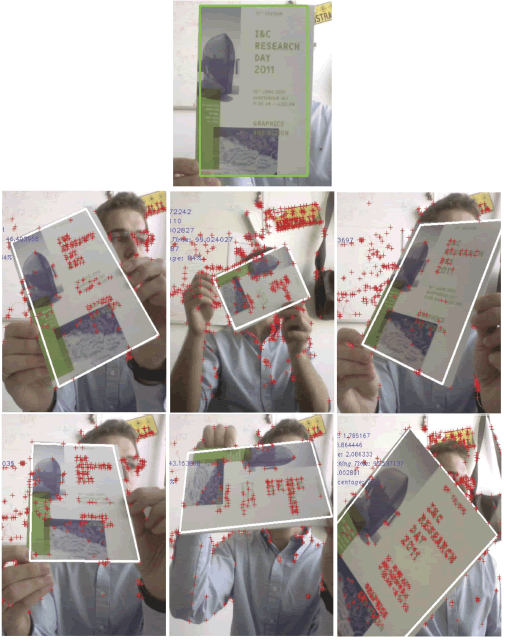
\includegraphics[width=.5\textwidth]{imgs/figure17.png} 
       \end{center} 
      }


\subsection{Conclusion}
\frame{ \frametitle{Conclusion}
  \begin{center}
  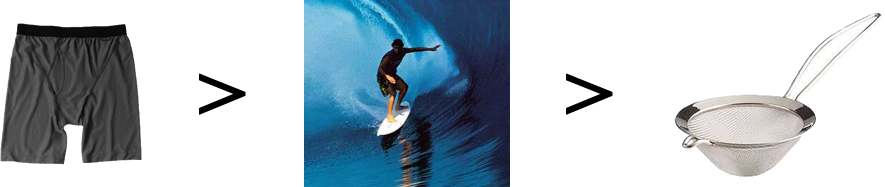
\includegraphics[width=1.0\textwidth]{imgs/conclusion.png}
  \end{center}
}

\subsection{References}
\frame{ \frametitle{References}
\begin{center}
 \begin{itemize}
  \item http://www.embege.com/gauss/
  \item http://cvlab.epfl.ch/~strecha/multiview/denseMVS.html
  \item http://www.cs.ubc.ca/~mbrown/patchdata/patchdata.html
  \item http://www.robots.ox.ac.uk/~vgg/research/affine/
  \item Dr. Gunturk's "Machine Recognition of Patterns" class notes
 \end{itemize}
\end{center}
}

\end{document}



